\chapter{一元函数的积分}
\label{chap:univariate-integration}

速度随时间变化时，一段时间内走过的路程是多少？上一章研究了已知函数时怎样求变化率，本章研究反方向的问题：已知各处的变化率或密度，怎样累计成总量。
有限和已经能处理分段常数的情形，一般情形需要把区间切得越来越细，看有限累计能否稳定到一个确定的数。

本章先用区间分割上的有限和定义黎曼积分，给出可积性的判别和积分的基本性质。
微积分基本定理接着说明，累计函数的变化率就是被积函数，因而定积分可以用原函数计算；换元与分部积分则把已知的原函数用于新的被积函数。

随后把积分推广到无穷区间与无界函数，研究积分与极限何时可以交换，最后用带权的有限和近似积分并比较几种求积公式的误差。
本章限于实区间上的黎曼积分。每次交换积分与极限，都要说明控制误差的条件；反常积分则另外检查端点或无穷远处的收敛。

\section{定积分的定义与性质}
\label{sec:ru-riemann-integral}

\subsection{黎曼和}
\label{sec:ru-riemann-sums}

速度恒为$v$时，时长$\Delta t$内的位移是$v\,\Delta t$。速度随时间变化时，可以把时间区间切成许多小段，每段内速度变化不大，就用该段某一时刻的速度乘以段长近似这一段的位移，再把各段加起来。
同样的做法用于曲线下的面积：把底边切成小段，每段用一个矩形近似。下面把这个过程写成一般的定义。

设$f$定义在$[a,b]$上。取有限个分点$a=x_0<x_1<\cdots<x_n=b$，称为$[a,b]$的一个\term{分割}（partition）$P$，记$\Delta x_i=x_i-x_{i-1}$，并称最长小段的长度$\|P\|=\max_i\Delta x_i$为分割的网格尺度。
在每段中任取一点$\xi_i\in[x_{i-1},x_i]$，称和
\[
 S(f,P,\xi)=\sum_{i=1}^nf(\xi_i)\,\Delta x_i
\]
为一个\term{黎曼和}（Riemann sum）。$f\geq0$时每一项是一个矩形的面积；$f$取负值时，横轴下方的矩形按负号计入，所以黎曼和是带符号的累计。
黎曼和依赖两种选择：分割$P$与取样点$\xi$。让$\|P\|\to0$是要求每一段都变短，而不只是增加分点的个数。

\begin{definition}[黎曼积分]
\label{def:ru-riemann-integral}
设$f:[a,b]\to\mathbb R$有界。若存在实数$A$，使对每个$\varepsilon>0$都存在$\delta>0$，只要$\|P\|<\delta$，无论怎样选取样点都有$|S(f,P,\xi)-A|<\varepsilon$，
就称$f$在$[a,b]$上\term{黎曼可积}（Riemann integrable），称$A$为它的定积分，记作$\int_a^bf(x)\,\mathrm dx$。
\end{definition}
定义同时控制了全部足够细的分割与全部取样方式。只检查某一列等距分割配某种取样点是不够的：在$[0,1]$上，有理点取$1$、无理点取$0$的指示函数$\mathbb I_{\mathbb Q}$，
若总取等距分割的中点（中点都是有理数），黎曼和恒为$1$；若取样点全选无理数，黎曼和恒为$0$。两种取样都能任意细，却给出不同的结果，所以这个函数不黎曼可积。
积分变量只在积分号内部使用，换名不改变结果：$\int_a^bf(x)\,\mathrm dx=\int_a^bf(t)\,\mathrm dt$。

定积分是带符号的累计，不同于几何面积。$\int_0^{2\pi}\sin x\,\mathrm dx=0$，因为横轴上下两部分相互抵消；而正弦曲线与横轴围成的几何面积是$\int_0^{2\pi}|\sin x|\,\mathrm dx=4$。
图~\ref{fig:ru-riemann-sums}(a)画出了一个取样点不规则、分割不等距的黎曼和，负值部分以红色计入。

\begin{figure*}[!htbp]
 \centering
 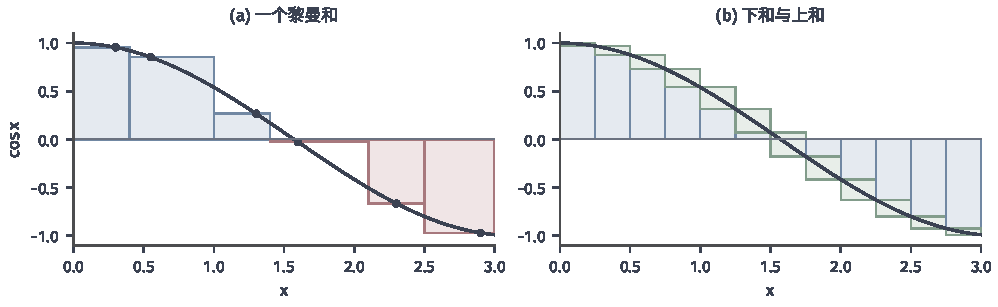
\includegraphics[width=169mm]{figures/01-basic-mathematics/02-real-numbers-and-univariate-functions/matplotlib/riemann-sums/figure.pdf}
 \caption{$f(x)=\cos x$在$[0,3]$上的累计。(a)不等距分割（$6$段）的一个黎曼和，黑点为各段的取样点，蓝色矩形按正号计入，红色矩形按负号计入。(b)同一函数在$12$段等距分割上的下和与上和：蓝色为下和，加上绿色部分得到上和，绿色总面积就是$U-L$。分割加细时这一差值趋于零，函数可积。图为解析示例。}
 \label{fig:ru-riemann-sums}
\end{figure*}

\subsection{可积性}
\label{sec:ru-integrability}

直接检查所有分割和取样并不方便。把每一段上可能的取样值夹在上下确界之间，就能用两个与取样无关的和控制全部黎曼和。
设$f$在$[a,b]$上有界，对分割$P$，记$m_i,M_i$为$f$在$[x_{i-1},x_i]$上的下确界与上确界，定义下和与上和
\[
 L(f,P)=\sum_im_i\,\Delta x_i,\qquad U(f,P)=\sum_iM_i\,\Delta x_i.
\]
同一分割下的任意黎曼和都满足$L(f,P)\leq S(f,P,\xi)\leq U(f,P)$。这里用确界而不用最值，因为有界函数在小段上未必取到最值。

加入新的分点时，一段被拆成几段，每个子段上的下确界不小于原段的下确界，上确界不大于原段的上确界，所以下和不减、上和不增。
任意两个分割有公共加细，因此任意下和都不超过任意上和。于是下积分$\sup_PL(f,P)$不超过上积分$\inf_PU(f,P)$。
\begin{theorem}[Darboux判据]
\label{thm:ru-darboux-criterion}
有界函数$f$在$[a,b]$上黎曼可积，当且仅当对每个$\varepsilon>0$，存在分割$P$使$U(f,P)-L(f,P)<\varepsilon$。此时积分等于上积分和下积分的共同值。
\end{theorem}
\begin{proof}
设条件成立。固定一个满足$U(f,P_0)-L(f,P_0)<\varepsilon$的分割$P_0$，设它有$k$个内分点，且$|f|\leq M$。对另一个分割$Q$，不含$P_0$分点的小段落在$P_0$的某一段内，沿用该段的上下界；
含有$P_0$分点的小段至多$k$个，总长度至多$k\|Q\|$，函数在其上的振幅至多为$2M$。所以$U(f,Q)-L(f,Q)\leq\varepsilon+2Mk\|Q\|$，$\|Q\|$足够小时小于$2\varepsilon$。
任意黎曼和与上下积分的共同值都夹在$L(f,Q)$与$U(f,Q)$之间，两者之差小于$2\varepsilon$，这正是黎曼可积的定义。
反过来，若$f$可积，取足够细的分割，在每段上分别取接近上确界与接近下确界的取样点，两组黎曼和都接近积分值，又分别接近$U$与$L$，所以$U-L$可以任意小。
\end{proof}
判据只用到实数的确界与有限分割，不需要事先知道积分值。图~\ref{fig:ru-riemann-sums}(b)中的绿色部分就是$U-L$。

\paragraph{可积函数类}
由判据可以判定几类函数可积。闭区间上的连续函数一致连续，给定$\varepsilon>0$，取$\delta$使距离小于$\delta$的两点函数值相差小于$\varepsilon/(b-a)$；

网格尺度小于$\delta$时每段的振幅$M_i-m_i<\varepsilon/(b-a)$，所以$U-L<\varepsilon$。
单调函数也可积：若$f$单调不减，取$n$等分，$M_i=f(x_i)$、$m_i=f(x_{i-1})$，求和相消得$U-L=(f(b)-f(a))(b-a)/n\to0$。
只有有限个间断点的有界函数同样可积：用总长度很小的有限个区间把间断点隔开，这部分对$U-L$的贡献不超过$2M$乘以总长度，其余部分按连续函数处理。

可积性有真实的限制。前面的$\mathbb I_{\mathbb Q}$在$[0,1]$的每个小区间上都同时取到$0$和$1$，所以对任意分割$L=0$、$U=1$，差值不随分割加细而减小，Darboux判据不成立。
困难不在于分割不够细，而在于函数在任意短的区间内都剧烈振荡。这说明有界性本身不足以保证黎曼可积；上下和之间的差必须能随分割加细而趋于零。

\subsection{积分的性质}
\label{sec:ru-integral-properties}

以下性质都从黎曼和直接得到。若$f,g$在$[a,b]$上可积，对同一分割和同一组取样点，$S(\alpha f+\beta g,P,\xi)=\alpha S(f,P,\xi)+\beta S(g,P,\xi)$，取极限便得线性
\[
 \int_a^b(\alpha f+\beta g)=\alpha\int_a^bf+\beta\int_a^bg.
\]
对$a<c<b$，把$c$作为分点，左右两段的黎曼和相加就是全区间的黎曼和，于是$\int_a^bf=\int_a^cf+\int_c^bf$。约定$\int_b^af=-\int_a^bf$、$\int_a^af=0$后，这个等式对$a,b,c$的任意顺序都成立。
若$f\leq g$，每个黎曼和都保持这一大小关系，所以$\int_a^bf\leq\int_a^bg$。$|f|$也可积，因为它在每段上的振幅不超过$f$的振幅；由$-|f|\leq f\leq|f|$得$\bigl|\int_a^bf\bigr|\leq\int_a^b|f|$。
乘积$fg$也可积，但积的积分一般不等于积分的积：在$[0,1]$上$\int x\cdot x\,\mathrm dx=1/3$，而$(\int x\,\mathrm dx)^2=1/4$。

\paragraph{误差估计与积分平均值}
保序性给出两个后面反复使用的估计。第一个是误差估计：若$|f-g|\leq\eta$在$[a,b]$上处处成立，则
\[
 \Bigl|\int_a^bf-\int_a^bg\Bigr|\leq\int_a^b|f-g|\leq\eta\,(b-a),
\]
函数的统一误差界乘以区间长度，就是积分的误差界。第~\ref{sec:ru-limit-interchange}节用它交换极限与积分，第~\ref{sec:ru-numerical-quadrature}节用它估计求积误差。
第二个是积分平均值：若$f$在$[a,b]$上连续，$m\leq f\leq M$分别为最小值与最大值，则$m\leq\frac1{b-a}\int_a^bf\leq M$，由介值定理，存在$c\in[a,b]$使
\[
 \int_a^bf(x)\,\mathrm dx=f(c)\,(b-a).
\]
$\frac1{b-a}\int_a^bf$称为$f$在$[a,b]$上的平均值，它是有限个函数值的算术平均在连续情形下的对应物。
\section{微积分基本定理}
\label{sec:ru-fundamental-theorem}

求导记录局部变化，积分记录一段范围内的累计。两者能否相互恢复，要分两个方向回答：对累计函数求导能否得到被积函数；对导数积分能否得到原函数的增量。

\subsection{累计函数的变化率}
\label{sec:ru-accumulation-derivative}

设$f$在$[a,b]$上可积，固定积分起点$a$，令
\[
 F(x)=\int_a^xf(t)\,\mathrm dt,\qquad a\leq x\leq b,
\]
称为$f$的累计函数，$t$是积分变量，$x$是$F$的自变量。若$|f|\leq M$，由区间可加性与绝对值估计，$|F(y)-F(x)|=\bigl|\int_x^yf\bigr|\leq M|y-x|$，所以累计函数总是Lipschitz连续的。
差商$(F(x+h)-F(x))/h=\frac1h\int_x^{x+h}f$恰是$f$在短区间上的平均值。若$f$在该点连续，短区间上的平均值应趋于该点的函数值。
\begin{theorem}[累计函数的导数]
\label{thm:ru-accumulation-derivative}
设$f$在$[a,b]$上可积，$F(x)=\int_a^xf$。若$f$在$c\in(a,b)$处连续，则$F'(c)=f(c)$；在端点处连续时，相应的单侧导数等于端点值。特别地，若$f$在$[a,b]$上连续，则$F'=f$处处成立。
\end{theorem}
\begin{proof}
对充分小的$h\neq0$，
\[
 \Bigl|\frac{F(c+h)-F(c)}h-f(c)\Bigr|=\Bigl|\frac1h\int_c^{c+h}\bigl(f(t)-f(c)\bigr)\,\mathrm dt\Bigr|\leq\sup_{|t-c|\leq|h|}|f(t)-f(c)|,
\]
由$f$在$c$处连续，右侧随$h\to0$趋于零。
\end{proof}
这里有三种强弱不同的结论：累计函数总是连续的；它在被积函数的连续点可微，导数等于函数值；被积函数处处连续时，可以保证它在区间内部处处可微，端点处具有相应的单侧导数。连续性在这里是充分条件；若不作这一假设，结论可能不成立，下面的两个例子分别说明导数不存在和导数不等于被积函数值的情形。
在$[-1,1]$上取阶跃函数$f=\mathbb I_{[0,1]}$，它只有一个间断点，因而可积，累计函数为$F(x)=\int_{-1}^xf=\max\{x,0\}$。在$x\neq0$处$F'=f$，在$x=0$处左差商恒为$0$、右差商恒为$1$，$F'(0)$不存在。
在间断点处，导数也可能存在却不等于函数值：把$f$取为只在$0$处等于$1$、其余处为$0$的函数，它的累计函数恒为零，$F'(0)=0\neq f(0)$。

\subsection{由原函数计算积分}
\label{sec:ru-newton-leibniz}

上一小节从积分出发得到导数。反过来，若已经知道一个函数的导数是$f$，能否用它计算$f$的积分？
设$f$定义在区间$I$上，若可微函数$G$在$I$上满足$G'=f$，就称$G$为$f$的\term{原函数}（antiderivative）。两个原函数的差的导数为零，由中值定理，它们在同一区间上只相差一个常数。
\begin{theorem}[Newton--Leibniz公式]
\label{thm:ru-newton-leibniz}
设$f$在$[a,b]$上连续，$G$是它在$[a,b]$上的任一原函数，则
\[
 \int_a^bf(x)\,\mathrm dx=G(b)-G(a)=:\bigl[G(x)\bigr]_a^b.
\]
\end{theorem}
\begin{proof}
由定理~\ref{thm:ru-accumulation-derivative}，累计函数$F(x)=\int_a^xf$也是$f$的原函数，所以$G=F+C$。于是$G(b)-G(a)=F(b)-F(a)=\int_a^bf$。
\end{proof}
这个公式把求定积分化为求原函数：例如$(x^3/3)'=x^2$，所以$\int_0^1x^2\,\mathrm dx=1/3$，与图~\ref{fig:ru-riemann-sums}中上下和夹逼的数值一致。

被积函数连续只是一个方便的充分条件。若$G$在$[a,b]$上连续、在$(a,b)$内可导，并且$G'$在$[a,b]$上黎曼可积（端点处任取有限值），则同样有$\int_a^bG'=G(b)-G(a)$。
证明直接用中值定理：对任意分割，在每段上选$\xi_i$使$G(x_i)-G(x_{i-1})=G'(\xi_i)\Delta x_i$，于是$G(b)-G(a)=\sum_iG'(\xi_i)\Delta x_i$恰好是一个黎曼和，令网格尺度趋零，它趋于$\int_a^bG'$。

\paragraph{原函数与可积性}
三个概念需要分开：有原函数、黎曼可积、原函数能用基本函数写出。阶跃函数$\mathbb I_{[0,1]}$在$[-1,1]$上可积，却没有原函数：若$G'=f$，则$G$在$[-1,0]$上为常数、在$[0,1]$上为$x$加常数，在$0$处左导数为$0$、右导数为$1$，与$G'(0)=1$矛盾。
连续函数总有原函数，即它的累计函数；但原函数未必能用基本函数经有限次运算写出。$e^{-x^2}$就是这样的例子（其证明超出本书范围），它的原函数通常直接写成累计函数$\int_0^xe^{-t^2}\,\mathrm dt$。
因此，使用这一方向的基本定理时，必须同时核对原函数的可微性和导数的黎曼可积性。
\section{积分的计算}
\label{sec:ru-integration-methods}

微积分基本定理把定积分的计算化为寻找原函数。本节先由导数表整理基本函数的原函数，再说明换元与分部积分怎样利用已知的原函数处理新的被积函数。

\subsection{基本函数的积分}
\label{sec:ru-basic-antiderivatives}

把导数表倒过来读，就得到基本函数的原函数。在所注明的区间上，
\[
 \begin{aligned}
 &\int x^\alpha\,\mathrm dx=\frac{x^{\alpha+1}}{\alpha+1}+C\ (\alpha\neq-1),&&\int\frac{\mathrm dx}x=\log|x|+C\ (x\neq0),\\
 &\int e^x\,\mathrm dx=e^x+C,&&\int a^x\,\mathrm dx=\frac{a^x}{\log a}+C\ (a>0,\ a\neq1),\\
 &\int\sin x\,\mathrm dx=-\cos x+C,&&\int\cos x\,\mathrm dx=\sin x+C,\\
 &\int\frac{\mathrm dx}{1+x^2}=\arctan x+C,&&\int\frac{\mathrm dx}{\sqrt{1-x^2}}=\arcsin x+C\ (|x|<1).
 \end{aligned}
\]
幂函数的公式在$\alpha=-1$时分母为零，这一情形单独由对数给出；$\log|x|$在$x<0$时的导数为$\frac{1}{-x}\cdot(-1)=\frac1x$，所以公式在两侧都成立。$x^\alpha$的允许区间与第~\ref{sec:ru-elementary-derivatives}节相同。

记号$\int f(x)\,\mathrm dx=G(x)+C$称为\term{不定积分}（indefinite integral），它表示$f$在一个区间上的全部原函数组成的一族函数，$C$取遍实常数；定积分$\int_a^bf$则是一个数。

若定义域由互不相连的几个区间组成，每个区间上可以取不同的常数，例如$1/x$在$(-\infty,0)$与$(0,+\infty)$上的原函数可以各取一个常数。
线性性质把复杂的被积函数拆成基本函数，例如
\[
 \int_1^2\Bigl(3x^2-\frac2x\Bigr)\,\mathrm dx=\bigl[x^3-2\log x\bigr]_1^2=7-2\log2.
\]

求出原函数后，可以求导回代核对，再检查积分区间是否落在公式成立的范围内。若忽略这一步，会得到错误的结果：$\int_{-1}^1x^{-2}\,\mathrm dx$按$[-1/x]_{-1}^1$计算得$-2$，
可是被积函数为正，积分不可能为负。问题在于$x^{-2}$在$0$处无界，不满足Newton--Leibniz公式的条件；这个积分要按第~\ref{sec:ru-improper-integrals}节的反常积分处理，实际上是发散的。

\subsection{换元法}
\label{sec:ru-substitution}

链式法则给出复合函数的导数，倒过来就是换元积分。
\begin{theorem}[换元公式]
\label{thm:ru-substitution}
设$\varphi$在$[\alpha,\beta]$上连续可微，$f$在包含$\varphi([\alpha,\beta])$的区间上连续，则
\[
 \int_{\varphi(\alpha)}^{\varphi(\beta)}f(u)\,\mathrm du=\int_\alpha^\beta f(\varphi(t))\,\varphi'(t)\,\mathrm dt.
\]
\end{theorem}
\begin{proof}
设$F$是$f$的原函数。由链式法则，$(F\circ\varphi)'=f(\varphi)\varphi'$，右侧被积函数连续，所以由Newton--Leibniz公式右边等于$F(\varphi(\beta))-F(\varphi(\alpha))$，左边也等于这个数。
\end{proof}
公式中的微分因子与积分端点一同变化：$\mathrm du$换成$\varphi'(t)\,\mathrm dt$，反映输入区间长度的伸缩；端点换成$\varphi$的对应值。定理不要求$\varphi$单调，$\varphi'<0$时端点的先后颠倒，由有向积分的约定自动处理符号。
例如$\int_0^12xe^{x^2}\,\mathrm dx$的被积函数形如$f(\varphi(x))\varphi'(x)$，取$\varphi(x)=x^2$、$f(u)=e^u$，得$\int_0^1e^u\,\mathrm du=e-1$。

另一种用法是引入新变量化简被积函数，这时要选定反函数的分支。计算四分之一单位圆的面积$\int_0^1\sqrt{1-x^2}\,\mathrm dx$，令$x=\sin\theta$。
新变量的范围取$[0,\pi/2]$，它使$\sin$从$0$递增到$1$，端点对应$0\mapsto0$、$\pi/2\mapsto1$，方向不变。在这一范围内$\cos\theta\geq0$，所以$\sqrt{1-\sin^2\theta}=\cos\theta$，开方不带负号。于是
\[
 \int_0^1\sqrt{1-x^2}\,\mathrm dx=\int_0^{\pi/2}\cos^2\theta\,\mathrm d\theta=\Bigl[\frac\theta2+\frac{\sin2\theta}4\Bigr]_0^{\pi/2}=\frac\pi4,
\]
其中用到$\cos^2\theta=(1+\cos2\theta)/2$。若把范围取成$[\pi/2,\pi]$，$\cos\theta\leq0$，开方必须写成$-\cos\theta$，同时端点方向也颠倒，结果仍是$\pi/4$；忽略其中一项就会出错。
这里的换元依赖上述连续性和可微性条件，不能只凭形式相同就替换变量。

\subsection{分部积分法}
\label{sec:ru-integration-by-parts}

乘积的导数$(uv)'=u'v+uv'$含有两项。对它积分并移项，就能把其中一项的积分换成另一项。
\begin{theorem}[分部积分公式]
\label{thm:ru-integration-by-parts}
设$u,v$在$[a,b]$上连续可微，则
\begin{equation}
 \int_a^bu(x)v'(x)\,\mathrm dx=\bigl[u(x)v(x)\bigr]_a^b-\int_a^bu'(x)v(x)\,\mathrm dx.
 \label{eq:ru-integration-by-parts}
\end{equation}
\BookEquationAliases{\label{eq:analysis-integration-by-parts}}
\end{theorem}
\begin{proof}
由乘积法则，$uv$在$[a,b]$上连续可微且$(uv)'=u'v+uv'$，右侧两项都连续。由Newton--Leibniz公式，$\int_a^b(u'v+uv')=u(b)v(b)-u(a)v(a)$，再由积分的线性移项即得。
\end{proof}

使用时把被积函数拆成$u$与$v'$两个因子：求导后变简单的因子取作$u$，容易找到原函数的因子取作$v'$。


计算$\int_0^1xe^x\,\mathrm dx$，取$u=x$、$v'=e^x$，则$u'=1$、$v=e^x$，于是结果为$[xe^x]_0^1-\int_0^1e^x\,\mathrm dx=e-(e-1)=1$；边界项$[xe^x]_0^1=e$不能遗漏。
只有一个因子时，可以把$1$当作另一个因子：$\int_1^e\log x\,\mathrm dx$取$u=\log x$、$v'=1$，得$[x\log x]_1^e-\int_1^e1\,\mathrm dx=e-(e-1)=1$。
若反过来分配，例如对$\int x\sin x\,\mathrm dx$取$u=\sin x$、$v'=x$，剩下的积分含$x^2\cos x$，反而更复杂。

\paragraph{Taylor公式的积分余项}
分部积分的一个重要应用，是把Taylor公式的余项写成积分，从而去掉Lagrange余项中位置未知的中间点。设$f$在包含$a$与$a+h$的区间上$n+1$阶连续可微，令$\phi(t)=f(a+th)$，$t\in[0,1]$，则$\phi^{(k)}(t)=h^kf^{(k)}(a+th)$。
从$\phi(1)-\phi(0)=\int_0^1\phi'(t)\,\mathrm dt$出发，对$k\geq1$，在$\int_0^1\frac{(1-t)^{k-1}}{(k-1)!}\phi^{(k)}(t)\,\mathrm dt$中取$u=\phi^{(k)}$、$v=-(1-t)^k/k!$，分部积分给出
\[
 \int_0^1\frac{(1-t)^{k-1}}{(k-1)!}\phi^{(k)}(t)\,\mathrm dt=\frac{\phi^{(k)}(0)}{k!}+\int_0^1\frac{(1-t)^k}{k!}\phi^{(k+1)}(t)\,\mathrm dt.
\]
从$k=1$用到$k=n$，每一步分出一项$f^{(k)}(a)h^k/k!$，便得到带积分余项的Taylor公式
\begin{equation}
 f(a+h)=\sum_{k=0}^n\frac{f^{(k)}(a)}{k!}h^k+\frac{h^{n+1}}{n!}\int_0^1(1-t)^nf^{(n+1)}(a+th)\,\mathrm dt.
 \label{eq:ru-taylor-integral-remainder}
\end{equation}
\BookEquationAliases{\label{eq:analysis-taylor-integral-remainder}}
若$|f^{(n+1)}|\leq M$，由$\int_0^1(1-t)^n\,\mathrm dt=1/(n+1)$，余项不超过$M|h|^{n+1}/(n+1)!$，与第~\ref{sec:ru-taylor-remainders}节的Lagrange余项给出同样的界。
积分余项不含未知点，可以直接夹逼。取$f=e^x$、$a=0$、$h=1$，余项为$\frac1{n!}\int_0^1(1-t)^ne^t\,\mathrm dt$，由$1\leq e^t\leq e$，它介于$1/(n+1)!$与$e/(n+1)!$之间；
$n=3$时$e-8/3\approx0.0516$，确实落在$1/24$与$e/24$之间。第~\ref{sec:ru-numerical-quadrature}节估计求积公式的局部误差时，同样要用Taylor展开把误差归结为高阶导数的界。
\section{反常积分}
\label{sec:ru-improper-integrals}

黎曼积分只对有限区间上的有界函数定义。下面两个积分都不在这个范围内：$\int_1^\infty x^{-2}\,\mathrm dx$的积分区间无界；$\int_0^1x^{-1/2}\,\mathrm dx$的区间有限，被积函数却在$0$附近无界。
处理办法是先在一个有限、有界的部分上积分，再让这个部分扩大，看积分是否有极限。

\subsection{无穷区间与奇点处的截断极限}
\label{sec:ru-improper-definition}

设$f$在每个$[a,b]$（$b>a$）上可积。若$\lim_{b\to+\infty}\int_a^bf$存在且有限，就称\term{反常积分}（improper integral）$\int_a^{+\infty}f$收敛，并以这个极限为它的值；否则称发散。
例如$\int_1^bx^{-2}\,\mathrm dx=1-1/b\to1$，所以$\int_1^\infty x^{-2}\,\mathrm dx=1$；而$\int_1^bx^{-1}\,\mathrm dx=\log b\to+\infty$，$\int_1^\infty x^{-1}\,\mathrm dx$发散。
被积函数在端点附近无界时，先避开这个点再取单侧极限：若$f$在每个$[a+\varepsilon,b]$上可积，定义$\int_a^bf=\lim_{\varepsilon\to0^+}\int_{a+\varepsilon}^bf$。
例如$\int_\varepsilon^1x^{-1/2}\,\mathrm dx=2-2\sqrt\varepsilon\to2$。函数在端点附近无界的点称为奇点。

区间两端都无界，或者区间内部有奇点时，要在中间取一点把积分拆开，要求每一段分别收敛，再相加；结果不依赖拆分点的选择。
这一要求防止用抵消掩盖某一侧的发散。$\int_{-\infty}^{+\infty}x\,\mathrm dx$的对称截断$\int_{-b}^bx\,\mathrm dx$恒为零，但$\int_0^{+\infty}x\,\mathrm dx$发散，所以这个反常积分发散。
同样，$\int_{-1}^1x^{-1}\,\mathrm dx$在内部有奇点，两侧$\int_0^1x^{-1}\,\mathrm dx$与$\int_{-1}^0x^{-1}\,\mathrm dx$都发散，它也发散。
对称截断的极限称为Cauchy主值，上面两个积分的主值都是$0$。主值是另一种规定，在特定问题中有用，但不能当作通常反常积分的值。

\subsection{收敛判别、绝对收敛与尾部误差}
\label{sec:ru-improper-tests}

若$f\geq0$，$\int_a^bf$随$b$单调不减，所以$\int_a^\infty f$收敛当且仅当这些截断积分有上界，与非负项级数的情形相同。由此得到比较判别：
若$0\leq f\leq g$且$\int_a^\infty g$收敛，则$\int_a^\infty f$收敛。不要求非负时，用柯西准则：$\int_a^\infty f$收敛，当且仅当对每个$\varepsilon>0$，存在$B$使$b_2>b_1>B$时$\bigl|\int_{b_1}^{b_2}f\bigr|<\varepsilon$。
比较需要基准。由原函数直接计算，
\[
 \int_1^\infty x^{-p}\,\mathrm dx\ \text{收敛}\iff p>1,\qquad\int_0^1x^{-p}\,\mathrm dx\ \text{收敛}\iff p<1.
\]
两者方向相反：无穷远处需要衰减得足够快，零点附近则不能增长得太快。

收敛的反常积分可以用有限区间上的积分近似，误差就是剩下的尾部，比较判别同时给出它的上界。例如$\int_0^\infty e^{-x^2}\,\mathrm dx$：在$x\geq b>0$上$e^{-x^2}\leq(x/b)e^{-x^2}$，所以
\[
 0\leq\int_b^\infty e^{-x^2}\,\mathrm dx\leq\frac1b\int_b^\infty xe^{-x^2}\,\mathrm dx=\frac{e^{-b^2}}{2b}.
\]
截断到$[0,3]$时，尾部误差不超过$e^{-9}/6\approx2\times10^{-5}$。剩下的有限区间积分再用第~\ref{sec:ru-numerical-quadrature}节的求积公式计算。

\paragraph{绝对收敛与条件收敛}
若$\int_a^\infty|f|$收敛，称$\int_a^\infty f$绝对收敛。由柯西准则和$\bigl|\int_{b_1}^{b_2}f\bigr|\leq\int_{b_1}^{b_2}|f|$，绝对收敛蕴含收敛。反之不成立，$\int_1^\infty\frac{\sin x}x\,\mathrm dx$是代表例子。
对截断积分分部积分，取$u=1/x$、$v'=\sin x$，
\[
 \int_1^b\frac{\sin x}x\,\mathrm dx=\Bigl[-\frac{\cos x}x\Bigr]_1^b-\int_1^b\frac{\cos x}{x^2}\,\mathrm dx.
\]
$b\to\infty$时边界项趋于$\cos1$，右边的积分由$|\cos x|/x^2\leq1/x^2$绝对收敛，所以原积分收敛。但在每个$[k\pi,(k+1)\pi]$上$\int|\sin x|/x\geq\frac2{(k+1)\pi}$，累加起来是调和级数，所以$\int_1^\infty|\sin x|/x$发散。
这个积分的收敛来自正负部分的振荡抵消，称为条件收敛，与交错级数的情形相似。因此，反常积分收敛与绝对收敛必须分别判断，不能把前者当成后者。
\section{积分与极限的交换}
\label{sec:ru-limit-interchange}

用函数列逼近被积函数时，自然希望积分也随之收敛，即$\lim\int f_n=\int\lim f_n$。这是交换“积分”与“取极限”两个操作，和交换求导与极限一样，需要条件。

\subsection{函数列、级数与逐项积分}
\label{sec:ru-termwise-integration}

在固定的闭区间上，一致收敛足以保证交换。
\begin{theorem}[一致收敛与积分]
\label{thm:ru-uniform-limit-integral}
设每个$f_n$在$[a,b]$上黎曼可积，且$f_n$在$[a,b]$上一致收敛到$f$，则$f$在$[a,b]$上黎曼可积，并且$\int_a^bf_n\to\int_a^bf$。
\end{theorem}
\begin{proof}
给定$\varepsilon>0$，取$n$使$|f_n-f|<\varepsilon$处处成立。在每一小段上，$f$的上下确界与$f_n$的相差不超过$\varepsilon$，所以$U(f,P)-L(f,P)\leq U(f_n,P)-L(f_n,P)+2\varepsilon(b-a)$，
再取使$f_n$的上下和之差小于$\varepsilon$的分割，由Darboux判据$f$可积。积分的收敛来自误差估计：$\bigl|\int_a^bf_n-\int_a^bf\bigr|\leq(b-a)\sup_{[a,b]}|f_n-f|\to0$。
\end{proof}
证明的关键是“统一误差乘以区间长度”，所以区间必须有限，误差必须对所有$x$统一。逐点收敛不够，下面的窄峰说明了原因。
在$[0,1]$上令$f_n$在$[0,2/n]$上是以$(1/n,n)$为顶点的三角形，其余处为零（$n\geq2$）。每个三角形的面积都是$1$，所以$\int_0^1f_n=1$；

但对每个$x$，$f_n(0)=0$，而$x>0$时一旦$2/n<x$就有$f_n(x)=0$，所以$f_n$逐点收敛到$0$，积分的极限$1$不等于极限函数的积分$0$。
如图~\ref{fig:ru-narrow-spikes}所示，尖峰越来越窄、越来越高，总面积不变，却躲开了每一个固定的点；最大误差$\sup|f_n-0|=n$并不趋于零。

\begin{figure}[!htbp]
 \centering
 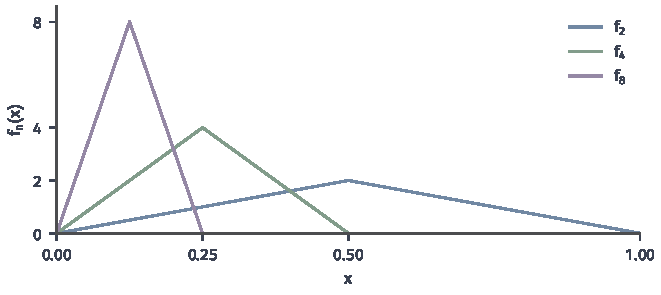
\includegraphics[width=112mm]{figures/01-basic-mathematics/02-real-numbers-and-univariate-functions/matplotlib/narrow-spikes/figure.pdf}
 \caption{窄峰函数列：$f_n$在$[0,2/n]$上为顶点$(1/n,n)$的三角形，其余处为零，图中画出$n=2,4,8$。每个三角形面积为$1$；固定任一$x>0$，$n>2/x$后$f_n(x)=0$，所以$f_n$逐点趋于零，积分却始终为$1$。图为解析示例。}
 \label{fig:ru-narrow-spikes}
\end{figure}

\paragraph{逐项积分}
把定理用于部分和：若各项$g_k$在$[a,b]$上可积，$\sum g_k$在$[a,b]$上一致收敛，则可以逐项积分，$\int_a^b\sum g_k=\sum\int_a^bg_k$。

幂级数在收敛区间内部的闭子区间上一致收敛，所以对$|x-x_0|<R$，
\[
 \int_{x_0}^x\sum_kc_k(t-x_0)^k\,\mathrm dt=\sum_k\frac{c_k}{k+1}(x-x_0)^{k+1},
\]
逐项积分后的级数仍以$R$为收敛半径。例如由几何级数$\frac1{1+t}=\sum(-t)^k$（$|t|<1$），在$[0,x]$上逐项积分，立即得到$\log(1+x)=\sum_{k\geq1}(-1)^{k+1}x^k/k$（$|x|<1$）；
对$\frac1{1+t^2}=\sum(-1)^kt^{2k}$逐项积分，得到$\arctan x$的展开。这为第~\ref{sec:ru-elementary-taylor}节用中值定理证明的两个展开提供了另一条路线，而且不需要估计余项。

这些结论都在有限闭区间上取得，不能直接推广为反常积分上的无条件交换：反常积分还多了一次截断的极限，需要另外控制。

\subsection{含参积分的连续与求导}
\label{sec:ru-parametric-integrals}

被积函数含有一个参数$y$时，积分$F(y)=\int_a^bf(x,y)\,\mathrm dx$是$y$的函数，称为含参积分。这里积分区间固定且有限，参数是唯一变化的实数。
$F$在$y_0$处是否连续，就是能否交换$y\to y_0$与积分。由上一小节的误差估计，若$y\to y_0$时$f(\cdot,y)$关于$x$一致趋于$f(\cdot,y_0)$，即$\sup_{x\in[a,b]}|f(x,y)-f(x,y_0)|\to0$，则$|F(y)-F(y_0)|\leq(b-a)\sup_x|f(x,y)-f(x,y_0)|\to0$，$F$在$y_0$处连续。
只在每个$x$处控制是不够的。把窄峰改写成连续参数：$y>0$时令$f(\cdot,y)$为$[0,2y]$上以$(y,1/y)$为顶点的三角形，$f(\cdot,0)\equiv0$。
对每个$x$，$y\to0^+$时$f(x,y)\to0$，但$y\leq1/2$时$F(y)=1$，而$F(0)=0$，$F$在$0$处不连续。

对参数求导也是一种极限交换。固定$x$，考察参数的差商$D_h(x)=[f(x,y+h)-f(x,y)]/h$，则$[F(y+h)-F(y)]/h=\int_a^bD_h(x)\,\mathrm dx$。
\begin{theorem}[积分号下求导]
\label{thm:ru-differentiation-under-integral}
设对$y$附近的每个参数，$f(\cdot,y)$在$[a,b]$上黎曼可积；并且$h\to0$时，$D_h$在$[a,b]$上一致收敛到某个函数$g$。则$F$在$y$处可导，且$F'(y)=\int_a^bg(x)\,\mathrm dx$。
\end{theorem}
\begin{proof}
任取一列$h_n\to0$，$D_{h_n}$在$[a,b]$上可积且一致收敛到$g$，由定理~\ref{thm:ru-uniform-limit-integral}，$g$可积且$\int D_{h_n}\to\int g$。由序列判据，差商$[F(y+h)-F(y)]/h\to\int g$。
\end{proof}
若$f$关于$y$可导，极限函数$g$就是偏导数$\partial f/\partial y$在$y$处的值，定理说的是$F'(y)=\int_a^b\frac{\partial f}{\partial y}(x,y)\,\mathrm dx$在差商一致收敛时成立。
以$F(y)=\int_0^1e^{xy}\,\mathrm dx$为例，参数只出现在指数因子中。由第~\ref{sec:ru-elementary-limits}节的估计$|e^u-1-u|\leq2u^2$（$|u|<1/2$），
\[
 \Bigl|D_h(x)-xe^{xy}\Bigr|=e^{xy}\Bigl|\frac{e^{xh}-1-xh}h\Bigr|\leq2e^{|y|}|h|,\qquad x\in[0,1],\ |h|<\tfrac12,
\]
所以差商关于$x$一致收敛，$F'(y)=\int_0^1xe^{xy}\,\mathrm dx$。$y\neq0$时可以直接核对：$F(y)=(e^y-1)/y$，两边都等于$(ye^y-e^y+1)/y^2$。
实际应用中更方便的充分条件是偏导数关于$(x,y)$连续，它需要多元函数的连续性，留到多元函数微积分部分（第~\ref{chap:multivariate-calculus}章）。
\section{数值求积}
\label{sec:ru-numerical-quadrature}

原函数不便求出，或者被积函数只能在有限个点上计算时，需要用有限和近似积分。黎曼和本身就是一种近似，但取样点和权重可以选得更好。
本节先确定加权积分这一对象，再分别构造矩形、梯形与Simpson公式，比较它们所需的光滑条件与误差。

\subsection{加权积分}
\label{sec:ru-weighted-integrals}

许多累计量带有权重：密度不均匀的细杆，总质量是密度乘以长度的累计；不同位置重要性不同的误差，总误差也要按位置加权。
设$w,f$在有限区间$[a,b]$上连续，称$\int_a^bw(x)f(x)\,\mathrm dx$为$f$关于权函数$w$的加权积分，$w(x)$描述位置$x$的权重。$w\equiv1$时回到普通积分。
若$w\geq0$且总权重$\int_a^bw>0$，则
\[
 \frac{\int_a^bw(x)f(x)\,\mathrm dx}{\int_a^bw(x)\,\mathrm dx}
\]
称为$f$的加权平均。由$\min f\leq f\leq\max f$乘以$w\geq0$再积分，它介于$f$的最小值与最大值之间，正如有限个数的加权平均介于最小数与最大数之间。

数值求积把积分近似为有限个函数值的加权和
\[
 \int_a^bf(x)\,\mathrm dx\approx\sum_{i=0}^nc_if(x_i),
\]
其中$x_i$称为节点，$c_i$称为求积系数。求积系数是有限个数，权函数$w$是区间上的函数，两者不要混淆；对加权积分求积时，$w$的影响会体现在系数中。
举一个连续加权平均的例子：在$[0,1]$上取$w(x)=2x$，总权重为$1$，$f(x)=x^2$的普通平均为$\int_0^1x^2\,\mathrm dx=1/3$，加权平均为$\int_0^12x\cdot x^2\,\mathrm dx=1/2$，权重偏向右端，平均值随之增大。
概率中的密度与期望正是这种计算，见\BookChapterRef{chap:random-variables}{卷2《数学准备：概率、因果与决策》的“随机变量与概率基础”章}。

下面的求积公式都把$[a,b]$等分为$n$段，步长$h=(b-a)/n$，节点$x_k=a+kh$，并用同一个算例$\int_0^1e^x\,\mathrm dx=e-1\approx1.718282$核对，取$n=4$。

\subsection{矩形求积}
\label{sec:ru-rectangle-rule}

最简单的做法是在每段上把$f$近似为常数，即用一个矩形代替这一段。取左端点、右端点或中点的函数值作为高，分别得到复合左矩形、右矩形与中点公式，例如
\[
 L_n=h\sum_{k=0}^{n-1}f(x_k),\qquad M_n=h\sum_{k=0}^{n-1}f\Bigl(x_k+\frac h2\Bigr).
\]
算例中$L_4=0.25\,(e^0+e^{0.25}+e^{0.5}+e^{0.75})\approx1.512437$，误差约$0.206$；$M_4=0.25\,(e^{0.125}+e^{0.375}+e^{0.625}+e^{0.875})\approx1.713815$，误差约$0.0045$。同样只用四个函数值，中点公式精确得多。

这些公式都是黎曼和，$f$连续时由一致连续性随$h\to0$收敛到积分。误差的阶取决于光滑条件。设$|f'|\leq M_1$，在第$k$段上$|f(x)-f(x_k)|\leq M_1(x-x_k)$，积分得局部误差不超过$M_1h^2/2$，$n$段相加得
\[
 \Bigl|L_n-\int_a^bf\Bigr|\leq\frac{M_1(b-a)}2h.
\]
中点公式多了一层抵消。设$|f''|\leq M_2$，在中点$m$处展开$f(x)=f(m)+f'(m)(x-m)+\frac12f''(\xi_x)(x-m)^2$，一次项关于中点对称，积分为零，剩下的不超过$\frac{M_2}2\int(x-m)^2=M_2h^3/24$，于是
\[
 \Bigl|M_n-\int_a^bf\Bigr|\leq\frac{M_2(b-a)}{24}h^2.
\]
端点公式的误差与$h$同阶，只需要一阶导数有界；中点公式的误差与$h^2$同阶，要求二阶导数有界。算例中两个上界分别为$e/8\approx0.34$与$e/384\approx0.0071$，都覆盖了实际误差。

\subsection{梯形求积}
\label{sec:ru-trapezoid-rule}

把每段上的$f$近似为连接两端函数值的直线，就得到梯形公式：第$k$段的积分近似为$\frac h2\bigl(f(x_k)+f(x_{k+1})\bigr)$。相加时内部节点被相邻两段共用，所以
\[
 T_n=h\Bigl[\frac12f(x_0)+f(x_1)+\cdots+f(x_{n-1})+\frac12f(x_n)\Bigr],
\]
端点系数为$h/2$，内部节点系数为$h$。算例中$T_4\approx1.727222$，误差约$0.0089$。

误差来自直线插值的偏差。设$p$是第$k$段上的直线插值，对段内固定的$x$，令$\phi(t)=f(t)-p(t)-K(t-x_k)(t-x_{k+1})$，选$K$使$\phi(x)=0$。$\phi$有$x_k,x,x_{k+1}$三个零点，两次用Rolle定理得某个$\xi$使$\phi''(\xi)=0$，即$K=f''(\xi)/2$。于是
\[
 |f(x)-p(x)|\leq\frac{M_2}2(x-x_k)(x_{k+1}-x),
\]
积分得局部误差不超过$\frac{M_2}2\cdot\frac{h^3}6=M_2h^3/12$，整体误差不超过$M_2(b-a)h^2/12$。
梯形公式与中点公式的误差都是$h^2$阶，所需条件相同，界的常数却是$1/12$对$1/24$；算例中梯形误差约为中点误差的两倍，且符号相反（梯形偏大、中点偏小），这正是凸函数的弦在图像之上、切线在图像之下。

\subsection{Simpson求积}
\label{sec:ru-simpson-rule}

用二次多项式代替直线，可以进一步提高精度。在长为$2h$的区间$[m-h,m+h]$上取端点与中点三个函数值$f_-,f_0,f_+$，过这三点的二次多项式$p(x)=A+B(x-m)+C(x-m)^2$满足$A=f_0$、$2Ch^2=f_-+f_+-2f_0$，积分得
\[
 \int_{m-h}^{m+h}p(x)\,\mathrm dx=2Ah+\frac23Ch^3=\frac h3\bigl(f_-+4f_0+f_+\bigr).
\]
中点的权重$4$来自二次项的积分。由对称性，奇次项的积分为零，所以这一公式对三次多项式也精确。把$[a,b]$分为偶数$n$段，每相邻两段组成一组，得到复合Simpson公式
\[
 S_n=\frac h3\bigl[f(x_0)+4f(x_1)+2f(x_2)+4f(x_3)+\cdots+2f(x_{n-2})+4f(x_{n-1})+f(x_n)\bigr],
\]
$n$必须是偶数，组与组之间的共用节点系数为$2h/3$。算例中$S_4\approx1.718319$，误差约$3.7\times10^{-5}$，同样只用了五个函数值。

若$f$的四阶导数连续且$|f^{(4)}|\leq M_4$，复合Simpson公式的误差满足
\[
 \Bigl|S_n-\int_a^bf\Bigr|\leq\frac{M_4(b-a)}{180}h^4,
\]
证明与梯形公式类似，用三点插值的误差估计，并利用对称性多抵消一阶\scite{math-suli2003numerical}。算例中上界为$e/(180\cdot256)\approx5.9\times10^{-5}$。

图~\ref{fig:ru-quadrature-rules}比较了三种公式：在相同的函数值数量下，Simpson公式的误差随$n$下降得最快，代价是需要更高阶的光滑性；被积函数只有低阶导数有界时，高阶公式的优势随之消失。

对反常积分，先按上一节的尾部估计截断到有限区间，再在有限区间上求积，总误差是两部分之和；被积函数在端点有奇点时，导数无界，上面的误差界都不能直接使用。

\begin{figure*}[!htbp]
 \centering
 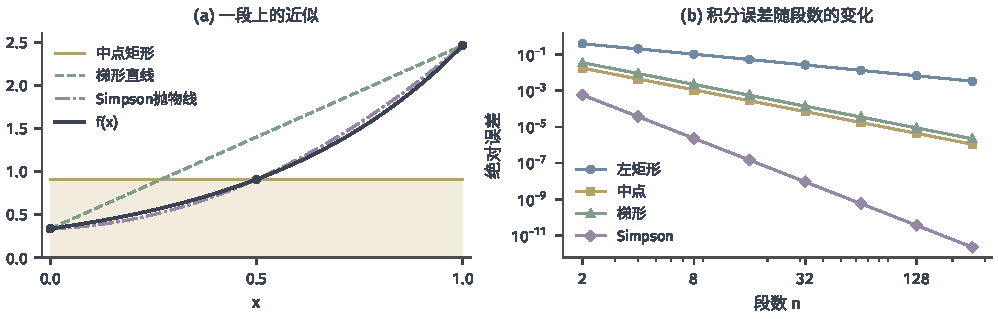
\includegraphics[width=169mm]{figures/01-basic-mathematics/02-real-numbers-and-univariate-functions/matplotlib/quadrature-rules/figure.pdf}
 \caption{三种求积公式的比较。(a)在一段$[0,1]$上近似$f(x)=e^{2x}/3$：中点公式用高为$f(1/2)$的矩形，梯形公式用连接两端的直线，Simpson公式用过两端与中点的抛物线，抛物线几乎与曲线重合。(b)$\int_0^1e^x\,\mathrm dx$的绝对误差随段数$n$变化，两轴均为对数刻度；左矩形、中点（与梯形）、Simpson的斜率分别约为$-1,-2,-4$，对应$h,h^2,h^4$阶误差。图为解析与双精度数值计算示例。}
 \label{fig:ru-quadrature-rules}
\end{figure*}

\FloatBarrier
\section{本章小结}
\label{sec:ru-integration-summary}

积分从有限累计出发：分割区间、在每段取样、乘以段长再求和，要求任意足够细的分割和任意取样都趋于同一个数。上下和把全部取样夹在中间，使可积性变成一个可以验证的误差条件；
连续函数、单调函数和只有有限个间断点的有界函数都可积，处处振荡的指示函数则不可积。

微积分基本定理把积分与导数联系起来：被积函数连续的点上，累计函数以它为导数；导数黎曼可积时，积分恢复端点增量。所以定积分可以由原函数计算，换元来自链式法则，分部积分来自乘积法则。

无穷区间和无界函数上的积分用截断再取极限定义，每一个问题点都要单独收敛，对称截断的抵消不能代替收敛；比较判别和幂函数基准给出尾部的误差界。

积分与极限的交换需要一致控制：在有限区间上一致收敛允许逐项积分，窄峰的例子说明逐点收敛不够；含参积分的连续与求导，也都要求参数附近的统一误差界。
数值求积用带权的有限和近似积分，矩形、梯形与Simpson公式的误差分别与步长的一次、二次和四次方成正比，前提是相应阶数的导数有界。

黎曼可积性和一致收敛的要求在两处显出了局限：逐点收敛的有界函数列，极限可能不再黎曼可积；有界函数在每个小区间上剧烈振荡时，分割无论多细都无法确定累计值。
这些局限也提出了进一步的问题：怎样测量更一般的集合，怎样定义更一般的积分，以及在什么条件下可以放宽一致收敛的要求。卷二的度量与测度部分将研究这些问题。
